%%%%%%%%%%%%%%%%%%%%%%%%%%%%%%%%%%%%%%%%%
% Journal Article
% LaTeX Template
% Version 1.3 (9/9/13)
%
% This template has been downloaded from:
% http://www.LaTeXTemplates.com
%
% Original author:
% Frits Wenneker (http://www.howtotex.com)
%
% License:
% CC BY-NC-SA 3.0 (http://creativecommons.org/licenses/by-nc-sa/3.0/)
%
%%%%%%%%%%%%%%%%%%%%%%%%%%%%%%%%%%%%%%%%%

%----------------------------------------------------------------------------------------
%   PACKAGES AND OTHER DOCUMENT CONFIGURATIONS
%----------------------------------------------------------------------------------------

\documentclass[twoside]{article}

\usepackage{lipsum} % Package to generate dummy text throughout this template

\usepackage[sc]{mathpazo} % Use the Palatino font
\usepackage[T1]{fontenc} % Use 8-bit encoding that has 256 glyphs
\linespread{1.05} % Line spacing - Palatino needs more space between lines
\usepackage{microtype} % Slightly tweak font spacing for aesthetics
\usepackage{listings}  

\usepackage[hmarginratio=1:1,top=32mm,columnsep=20pt]{geometry} % Document margins
\usepackage{multicol} % Used for the two-column layout of the document
\usepackage[hang, small,labelfont=bf,up,textfont=it,up]{caption} % Custom captions under/above floats in tables or figures
\usepackage{booktabs} % Horizontal rules in tables
\usepackage{float} % Required for tables and figures in the multi-column environment - they need to be placed in specific locations with the [H] (e.g. \begin{table}[H])
\usepackage{hyperref} % For hyperlinks in the PDF

\usepackage{lettrine} % The lettrine is the first enlarged letter at the beginning of the text
\usepackage{paralist} % Used for the compactitem environment which makes bullet points with less space between them
\usepackage{graphicx} % Used for including images
\usepackage{placeins}
\graphicspath{ {images/} }


\usepackage{abstract} % Allows abstract customization
\renewcommand{\abstractnamefont}{\normalfont\bfseries} % Set the "Abstract" text to bold
\renewcommand{\abstracttextfont}{\normalfont\small\itshape} % Set the abstract itself to small italic text

\usepackage{titlesec} % Allows customization of titles
\titleformat{\section}[block]{\large\scshape\centering}{\thesection.}{1em}{} % Change the look of the section titles
\titleformat{\subsection}[block]{\large}{\thesubsection.}{1em}{} % Change the look of the section titles

\usepackage{fancyhdr} % Headers and footers
\pagestyle{fancy} % All pages have headers and footers
\fancyhead{} % Blank out the default header
\fancyfoot{} % Blank out the default footer
\fancyhead[C]{CLI Messaging Application $\bullet$ April 2016 } % Custom header text
\fancyfoot[RO,LE]{\thepage} % Custom footer text

%----------------------------------------------------------------------------------------
%   TITLE SECTION
%----------------------------------------------------------------------------------------

\title{\vspace{-15mm}\fontsize{24pt}{10pt}\selectfont\textbf{CLI Messaging Application}} % Article title

\author{
\large
\textsc{Nir Boneh}\\[2mm] % Your name
\normalsize University of Colorado Boulder \\ % Your institution
\normalsize \href{mailto:nir.boneh@colorado.edu}{nir.boneh@colorado.edu} \\ % Your email address
\vspace{-5mm}
}
\date{}

%----------------------------------------------------------------------------------------

\begin{document}

\maketitle % Insert title

\thispagestyle{fancy} % All pages have headers and footers

%----------------------------------------------------------------------------------------
%   ABSTRACT
%----------------------------------------------------------------------------------------

\begin{abstract}

\noindent
This project discusses the creation and design of a decentralized CLI unix-based messaging application written in C. Examining 
closely on how to eliminate security risks and introspecting on the usefulness of the application in various situations. The 
advantages of using this application over other similar application in areas such as security, practicality, and speed is also 
discussed. Charts showing speed comparisons of sending messages over lan or wan are also shown. It also goes into detail about implementation and includes information on socket programming, hashmaps, and OpenSSL. The source code for the project can be found at \href{https://github.com/nboneh/CLIMessageApp}{https://github.com/nboneh/CLIMessageApp} and the repository can be used for downloading and installing the application.

\end{abstract}

%----------------------------------------------------------------------------------------
%   ARTICLE CONTENTS
%----------------------------------------------------------------------------------------

\begin{multicols}{2} % Two-column layout throughout the main article text

\section{Introduction}

\lettrine[nindent=0em,lines=3]{I}{}nstant messaging has become one of the most practical ways we communicate with one another. In this day and age, instead of having to send mail across the physical plane and
wait one to four business weeks to hear back from family relatives or friends, we can simply pull out our mobile device, type a 
message and send it in nearly an instant. While such power as reduced our face to face communication \cite{hemmer}, one can't deny the
advantages this tool could bring working within a unix terminal. For us developers and
UNIX enthusiasts, spending most of our time on a terminal managing files and building application; A CLI tool that allows messaging quickly from the 
terminal, would be nice to have added to our vast arsenal of gadgets that are within 
our efficient terminal fingertips. Not to mention such an application would be extremely practical in a situation where we are limited 
to just a terminal, such as with special types of machines or on remote ssh. While a great messaging CLI application does exist, 
called telegram \cite{telegram}, it does not serve the purpose of being a decentralized application. That means that big brother 
could be watching your messages not to mention that security attacks could happen to the the telegram server which is stated to be 
vulnerable to MITM (Man in the Middle) attacks according to a tech.eu article \cite{wauters}. The other risk is that the server could go offline 
rendering the application useless. There is also a chat application that is decentralized called chat terminal \cite{lanchat}. 
Installation for this application is diffcult and requires many pre requisite items and even after installing those I wasn't able to get it to compile. 
It also misses the key feature of messaging which is being able to save messaging history.  
So a messaging application that is decentralized, secure, and easy to install is missing from the terminal tool arsenal, which is the main focus of the CLI messaging 
application. 
%------------------------------------------------


\begin{figure*} % figure* spans two columns, figure is just one column
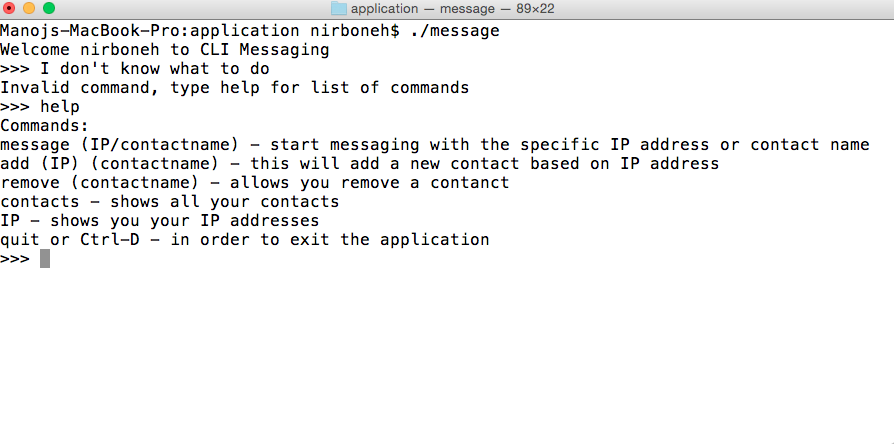
\includegraphics[width=1\textwidth,natwidth=894,natheight=444]{help.png}
\caption 
{The help command showing all available commands.}
\end{figure*}

\section{Design}

The CLI messaging application is written in C with over 1,000 lines of code and 800 lines of original code and is written for Unix based systems (Mac and Linux). It is easy to install, using git clone or downloading the source code from github and running make, it does however require that OpenSSL 1.0.xg is installed which might require more effort from Mac users. In this section we will go over the features and commands that CLI Messaging Application gives its users and a basic rundown of the commands implementation, a more detailed explnation of how the complex message command works will be covered in the implementation section. 

\subsection{The IP Command}

The IP command allows one to see his LAN and WAN IP addresses. This allows one to quickly share with his friends the way to contact him using the application. It works by having c call a small bash script using the system call that prints out the LAN and WAN IP to stdout.

\subsection{Contacts Commands}

There are three contacts commands that work to modify the same data. The add command allows one to add a new contact by typing in an IP address and a contact name. The remove command allow one to remove a contact based on his contact name. The contacts command allows one to see all of the current contacts. The contact data is store in a data structure called a hashmap which allows one to retrieve a value, in this case contact name, using a key, in this case IP address. An online open source project implementation hashmap was used for the application \cite{petewarden}. There is a forward and backward hashmap data structure one to look up IPs based on contact names and the other is to look up contact name based on IPs. The reason for this is if you want to send a message you will do so based on the contact name, and if you receive a message you will get the IP and need to know who it is from. The hashmap is saved on the disk in a text file and overwritten every time an add happens, remove happens, or the application exits, so the contacts are reloaded everytime the application is loaded. 

\subsection{Message Command}

The message command allows one to set up a messaging channel communication with another node based on their IP or contact name. Upon receiving the request, the second node decides whether to accept or reject the request. If the other node accepts both nodes will perform a secure handshake and enter message mode. This is where anything you type is sent over to the other user with a timestamp and the message, the entire conversation is always printed out. If one node types in quit, the application will go back to regular interactive mode, for both nodes. 
The message conversation is saved on disk based on the other node's IP and will be reloaded the next time a messaging channel is setup. 
The message command has the most complex implementation and will be discussed more in detail in the implementation section. 


\section{Implementation}
This section will go over socket communication and performing OpenSSL to send secure information between the two nodes. 
\subsection{Messaging between nodes }
A communication between two nodes is setup via TCP/IP connection using socket programming. Socket programming in C can be quite diffcult and confusing, so I would like to thank Beej's Guide to Network Programming for helping me setup the code \cite{hall}. Before communication channel is open a communication socket has to be setup and there are two ends to this. A connect socket and a listen socket, one request connection and the other accepts the connection. To set up a socket an IP address and a port is required, the application's port is set to be 3490 as macro in the code. The listen socket calls on the accept system call where it hangs till a connect socket requests connection. So how is it possible to run a listen socket without freezing the application? With the use of pthreading. The application sets up a listen socket on a seperate thread when it first boots up. Upon the accept socket system call returning a global is set up to let the UI thread know that a communication has been established. Once the link is performed sending of messages can be done via send and recv system calls, the recv system also hangs so again a second thread has to be setup. Everytime a user types in a message the send call is called and sends it to the receiver. Both the send and receive write to the same file, so a mutex lock is required to keep the resource safe since they run on seperate threads. A mutex lock works by only allowing one thread into a code section at a time making sure only one thread writes to the file. If one thread hangs up or quits the recv function returns a zero which lets the other end user know that the remote has hang up. This node sets a global to true in the receive thread and goes back to interactive mode. 
\subsection{Avoiding security risks}
There are two main security risks that are addressed when building the application. The first one is making sure to encrypt messages between two nodes so no one can decipher them, this is addressed using RSA through the use of a public key and private key. The second problem is being able to share the RSA public keys on a non-secure channel which is addressed using Diffie Hellman key exchange. The way that these algorithms are used in code pratice is through bash script calling on the OpenSSL library reading from a file and writing to a file. c calls on these bash scripts using the command function, writing to a file before and then reading from the output file, both files are then deleted using c's unlink system call. 
\subsubsection{RSA for secure communication}
The general idea of RSA works as follows, each user has a public key and a private key which they can generate using the RSA algorithm. Upon generating these two keys, a user can share his public key with 
everyone, but keeps 
the private key to himself. Now anyone who wants to share secure messages with another user, encrypts the message using the user public key, but the message can only be decrypted using the private key. Therefore, no 
one can read messages sent to the user other than the intended user himself. This is the main method of communication when two users are sending messages back and forth using the application. The RSA algorithm involves generating two large prime numbers and multiplying them togther to get a composite. In order for anyone to 
crack the RSA algorithm it would require being able to figure out the two prime numbers using factoring which is extremely diffcult and would take a ridicilous amount of time doing by brute force, so one can 
trust RSA to be a rather secure algorithm.
\subsubsection{Diffie Hellman key exchange}
The only issue with the RSA method alone is that the user needs to share his public key with another user on a non-secure channel and this 
is where security risks are prone, this is where Diffie Hellman key exchange comes into play. One possible security risk that could happen when sharing a public key on a non-secure channel is called Man in the Middle Attack. Let's imagine two users Alice and Bob, and a malicious user called Chris, here is how a man in the middle attack will play out:

\begin{enumerate}
  \item Bob sends a package to Alice: Hey Alice this is Bob, here is my public key: Bob's key.
  \item Chris intercepts the message and swaps out Bob's key with his own key.
  \item Alice receives the message and think that Bob's key is actually Chris's key.
  \item Alice sends back an encrypted message using Chris's key sharing her public key. 
  \item Chris intercepts that message as well, and decrypts it with his key and changes Alice's key to his key.
  \item Bob receives the message and assume Alice's key is Bob's key.
  \item From this point on Chris has got all the power over the conversation, being able to see it and also change it as he likes. 
\end{enumerate}

The only way to avoid such a terrible scenario is using the Diffie Hellman key exchange algorithm to share the public keys, the math is somewhat complicated, but the logic is rather simple and can be explained using colors:

\begin{enumerate}
  \item Bob and Alice share a public color which they both agree on, Chris can know about this public color.
  \item Bob and Alice both generate a private color neither one knows of the other and neither does Chris.
  \item Bob and Alice mix the public color with their private color and send it to each other, Chris can know about this color.
  \item Bob and Alice mix this color with their private color again and they both get the same color, now they both know a color that Chris doesn't know.
  \item Bob and Alice can now send the public key using this fourth color for encoding without Chris being able to manipulate the situation.
\end{enumerate}

While it is true that a man in the middle attack could disrupt the handshake, it will not be able to gain power over the conversation, since it can not know the fourth color. If a man in the middle attack those disrupt the process, the handshake can be retried over and over till he gets bored and moves on. The last component is using the secret known color to encrypt the RSA public key, this is done through an cipher algorithm called AES, which encrypts message based on a value and then the message can be decrypted using that same value. So, basically the way the application avoids security risks is by sharing public keys using Diffie Hellman and from there messages are exchanged using RSA.

\begin{table*}[t]
\centering
\begin{tabular}{ |p{3cm}||p{3cm}|p{3cm}|p{3cm}|  }
 \hline
 \multicolumn{4}{|c|}{Messaging Speed (Seconds)} \\
 \hline
Message Length& Telegram &CLI Messaging App LAN &CLI Messaging App WAN \\
 \hline
 Short (10 chars)   &0.764&0.376& 0.174\\
 Medium (30 chars)&0.768  &0.382& 0.188\\
 Long (75 chars) &0.774 & 0.383&0.199 \\
 \hline
\end{tabular}
\caption{ Shows speed comparison of CLI Messaging App on LAN and WAN network as well as telegram}
\end{table*}

\section{Evaluation}


\subsection{Methodology}
In order to compare the efficiency of the application, a speed comparison is done with well known CLI centralized messaging application called Telegram. The CLI messaging application is tested over WAN and LAN networks and the Telegram is tested normally, since you have to send a message through a server which makes it  WAN. The test is performed on short messages, medium messages, and long messages. To test the speed of messages on the CLI Messaging application a time shell script is called to print the time in milliseconds before RSA encryption and after the RSA decryption on the receiving end. The difference is then compared to get the speed. For the Telegram performane, what they like to call a bot is set up, and then using the bot send a message to my Telegram account is sent using CURL and then eveluated using the UNIX time command. 

\subsection{Results}
These are some strange results, but here is my theory on what happened.
When I was testing WAN I was testing my Mac communication with a Google Compute Engine Server and when I was testing on LAN I was testing my Linux VM and my Mac. So, the Google Compute Engine Server has less bottleneck in execution performance than the VM. My theory is that network I/O wasn’t the main culprit for speed execution, it was the RSA computation.
As for telegram being slower, I assume it is due to them having to run messaging through a centralized server and having to serve many clients.


%----------------------------------------------------------------------------------------
%   REFERENCE LIST
%----------------------------------------------------------------------------------------
\begin{thebibliography}{99} % Bibliography - this is intentionally simple in this template
\bibitem{hall}
Hall, Brian "Beej Jorgensen." Beej's Guide to Network Programming: Using Internet Sockets. Place of Publication Not Identified: Publisher Not Identified, 2009. Print.
\bibitem{hemmer}
Hemmer, Heidi. "Impact of Text Messaging on Communication." Minnesota State University, Mankato, 2009.
\bibitem{telegram}
"Telegram  a New Era of Messaging." Telegram. N.p., n.d.  \href{https://telegram.org/}{https://telegram.org/}
\bibitem{lanchat}
"LAN Chat and Text Conferencing in Easiest Way with Vypress Chat." Chat Terminal. N.p., n.d.  \href{http://www.vypress.com/free\textunderscore chat/}{http://www.vypress.com/free\textunderscore chat/}
\bibitem{malizia} 
Malizia, Nicola. "Getting Started with Telegram Bots." Unnikked. N.p., 25 June 2015. \href{https://unnikked.ga/getting-started-with-telegram-bots}{https://unnikked.ga/getting-started-with-telegram-bots}
\bibitem{petewarden}
"Petewarden c\_hashmap" GitHub. N.p., n.d.  \href{https://github.com/petewarden/c\_hashmap}{https://github.com/petewarden/c\_hashmap}
\bibitem{wauters}  
Wauters, Robin. "Supposedly Super Secure Telegram App Is Vulnerable to MITM Attacks, Cybersecurity Expert Claims." Tech.eu. N.p., 29 Apr. 2014.  \href{http://tech.eu/brief/supposedly-super-secure-telegram-app-possibly-vulnerable/}{http://tech.eu/brief/supposedly-super-secure-telegram-app-possibly-vulnerable/} 

\end{thebibliography}

%----------------------------------------------------------------------------------------

\end{multicols}

\end{document}

